\documentclass[10pt]{book}
\usepackage[a5paper,top=54pt,bottom=54pt,left=48pt,right=48pt]{geometry}
\usepackage[utf8]{inputenc}
\usepackage[T1,T2A]{fontenc}
\usepackage[english,russian]{babel}
\usepackage{graphicx}
\usepackage{amsmath,amsthm,amssymb}
\usepackage{caption2}
\usepackage{yhmath}



\linespread{0.5}

%page header
\usepackage{fancybox,fancyhdr}
\pagestyle{fancy}
\fancyhead{}
\fancyhead[LE,RO]{\textbf{\thepage}}
\fancyhead[RE]{\textit{\textsection 47. Криволинейные интегралы}}
\fancyhead[LO]{\textit{47.8 Интегралы, не зависящие от пути интегрирования}}
\fancyfoot{}
\renewcommand{\headrulewidth}{0pt}

\setcounter{page}{138}
\setcounter{figure}{149}

%remove colon after "Рис. %number%"
\renewcommand{\captionlabeldelim}{~}

%font
\fontfamily{lh}
\selectfont

\usepackage{pgfpages}
\pgfpagesuselayout{2 on 1}[a4paper,landscape,border shrink=5pt]


\begin{document}
	
	\noindent отображение $F$ мы наложили несколько более сильные условия,\linebreak
	потребовав непрерывности смешанных производных $\dfrac{d^2y}{du \ dv}$ и $\dfrac{d^2y}{dv \ du}$ и\linebreak
	возможности применения формулы Грина для области {Г*}). Нетрудно \linebreak
	убедиться и в том, что стремление к пределу в формуле (47.27) \linebreak
	происходит равномерно в смысле, указанном в теореме 1 п. 46.1 \par
	
	Несмотря на простоту вывода формулы (47.27), следует отметить, \linebreak
		что доказательство теоремы 1, приведенное в п. 46.1, идейно пред- \linebreak
		почтительнее, так как оно лучше раскрывает сущность вопроса, \linebreak
		связанную с тем, что дифференцируемое отображение в малом до- \linebreak
		статочно хорошо аппроксимируется линейным отображением. \par
	\begin{center}
		{\textbf{47.8. Криволинейные интегралы, не зависящие \linebreak от пути интегрирования}}
	\end{center}	
	
	
	\,\,\,\,Все кривые (контуры), рассматриваемые в этом пункте,\linebreak
	будут всегда предполагаться кусочно-гладкими; для краткости это\linebreak
	не будет каждый раз специально оговариваться.\par
	
	Рассмотрим вопрос о том, когда криволинейным интеграл \linebreak
	$\int\limits_{\wideparen{AB}} P dx + Q dy$ зависит только от точек A и B и не зависит от выбора \linebreak
	кривой $\wideparen{AB}$, их соединяющей. \par 
	
	\textit{\textbf{Теорема 3.} Пусть функции P(x, y) и Q(x, y) непрерывны в пло-\linebreak 
	ской области G, тогда эквивалентны следующие три условия.} \par
	
		
	 \textit{1. Для любого замкнутого контура $\gamma$, лежащего в G,} \par 
	
	$$ \int\limits_{\gamma} P dx + Q dy = 0.$$
	
	 \textit{2. Для любых двух точек A  $\in$ G и B $\in$ G значение интеграла} \linebreak 
	
	$$\int\limits_{\wideparen{AB}} P dx + Q dy$$
	
	\textit{не зависит от кривой $\wideparen{AB} \subset G$, соединяющей точки A и B.} \par 
	\textit{3. Выражение P dx + Q dy является в G полным дифференциалом,\linebreak
	т. е. существует функция u(M) = u(x, y), M = (x, y), определен-\linebreak
	ная в G и такая, что} \par
	
	$$du=P dx + Q dy. \eqno (47.28)$$
	\textit{В этом случае если A  $\in$ G и B $\in$ G, то}\par 
	
	$$ \int\limits_{\wideparen{AB}} P dx + Q dy = u \left( B \right) - u \left( A \right) \eqno (47.29)$$
	\textit{для любой кривой $\wideparen{AB}$, соединяющей в G эти точки.} \par 
	\textit{Таким образом, выполнение каждого из условий 1, 2 и 3 необходимо \linebreak и достаточно для выполнения каждого из двух остальных.} \par
	
	Д\,о\,к\,а\,з\,а\,т\,е\,л\,ь\,с\,т\,в\,о. Покажем, что из первого условия сле- \linebreak
	дует второе, из второго - третье, а из третьего - первое, т.е. про- \linebreak
	ведем доказательство по схеме \par 
	
	
	\begin{figure}[h]
        \begin{minipage}{1\textwidth}
	\centering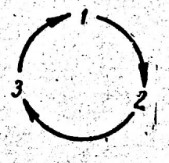
\includegraphics[width=60pt,height=100pt,keepaspectratio]{img1}
		\end{minipage}
	\end{figure}
	
	\noindent Этим будет, очевидно, доказано, что из любого условия 1, 2 и 3 следу- \linebreak
	ет любое другое из них. \par 
	
	\begin{figure}[h]
		\begin{minipage}{1.8\textwidth}
			\centering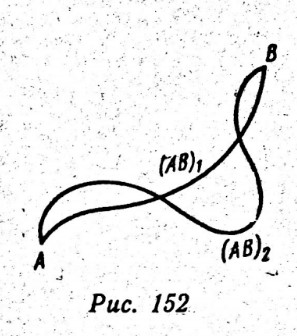
\includegraphics[width=60pt,height=60pt]{img2}
		\end{minipage}

	\end{figure}
	
	
	
	
	\noindent Но \par 
	$$\int\limits_{\left( \wideparen{AB} \right)_{1} \smile \left( \wideparen{BA} \right)_{2}} P dx + Q dy = \int\limits_{\left( \wideparen{AB} \right)_{1}} P dx + Q dy + 
	\int\limits_{\left( \wideparen{BA} \right)_{2}} P dx + Q dy =$$
	$$\int\limits_{\left( \wideparen{AB} \right)_{1}} P dx + Q dy - \int\limits_{\left( \wideparen{AB} \right)_{2}} P dx + Q dy.  \eqno (47.31)$$
	\noindent т.е. свойство 2 выполняется. \par 
	$$ $$\par 
	В\,т\,о\,р\,о\,й ш\,а\,г: 2 \to 3.$ Пусть M_{0}$ $\in$ G, M=(x, y) $\in$ G и $\wideparen{M_{0}M} -$ \linebreak
	некоторая кривая, соединяющая в G точки $M_{0}$ и M. \,Положим \par 
	$$ u(M)=\int\limits_{\wideparen{M_{0}M}} P dx + Q dy. $$ \par 
	В силу условия 2 при фиксированной точке $M_{0}$ функция u(x, y)\linebreak
	является однозначной функцией, так как значение u(M) = u(x, y) не \par 

\end{document}